\documentclass{standalone}
\usepackage{tikz}
\usepackage{ctex,siunitx}
\usepackage{tkz-euclide}
\usepackage{amsmath}
\usetikzlibrary{patterns, calc}
\usetikzlibrary {decorations.pathmorphing, decorations.pathreplacing, decorations.shapes,}
\begin{document}
\small
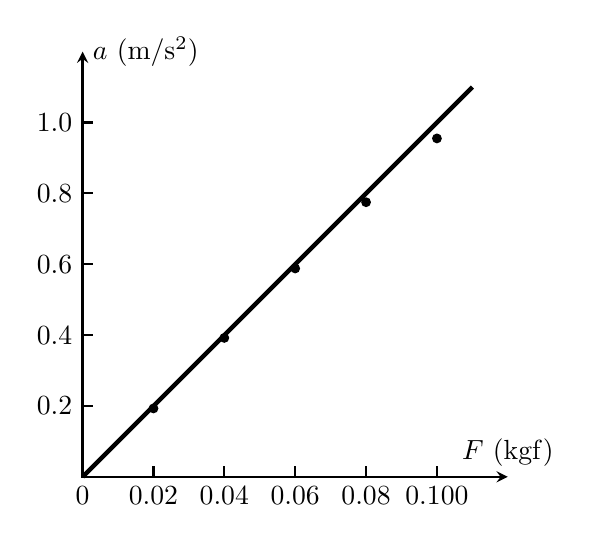
\begin{tikzpicture}[>=stealth,thick, scale=4.5]
  \draw [<->](0,1.2)node [right]{$a$ (\unit{m/s^2})}--(0,0)--(1.2,0)node [above]{$F$ (\unit{kgf})};
  \foreach \x in{1,2,3,4,5}
  {
      \draw(0,\x/5) --(0.03,\x/5);
      \draw(\x/5,0)--(\x/5,0.03);
  }
  \draw [fill=black] (0.020*10  ,  0.193)  circle [radius=.3pt];
  \draw [fill=black]  (0.040*10  ,  0.392 ) circle [radius=.3pt];
  \draw [fill=black]  (0.060*10  ,  0.588 ) circle [radius=.3pt];
  \draw [fill=black]  (0.080*10  ,  0.775)  circle [radius=.3pt];
  \draw [fill=black]  (0.100*10  ,  0.955)circle [radius=.3pt];
  \draw[ultra thick](0,0)--(1.1,1.1);
  \node at (0,0)[below]{0};
  \node at (0.2,0)[below]{0.02};
  \node at (0.4,0)[below]{0.04};
  \node at (0.6,0)[below]{0.06};
  \node at (0.8,0)[below]{0.08};
  \node at (1,0)[below]{0.100};
  \node at (0,0.2)[left]{0.2};
  \node at (0,0.4)[left]{0.4};
  \node at (0,0.6)[left]{0.6};
  \node at (0,0.8)[left]{0.8};
  \node at (0,1)[left]{1.0};
\end{tikzpicture}
\end{document}